\section{Цель работы}

Изучение основных характеристик свободных затухающих электромагнитных колебаний в колебательном контуре.

\section{Задачи работы}

\begin{enumerate}
    \item Измерение периода $T$ и амплитуд напряжения при различных $R_\text{М}$.
    \item Определение $\lambda$, $Q$, $R_0$ и $L$ контура.
    \item Исследование зависимости $T(C)$ и оценка $R_\text{кр}$.
\end{enumerate}

\section{Объект исследования}

Последовательный колебательный контур: катушка $L$, конденсатор $C$, магазин сопротивлений $R_\text{М}$.

\section{Метод эксперимента}

Наблюдение осциллограммы затухающих колебаний $U_C(t)$. Измерение периода и амплитуд, разделённых $n$ периодами.

\section{Измерительные приборы}

\begin{table}[h]
\centering
\caption{Список приборов}
\begin{tabular}{|l|l|p{5cm}|p{4cm}|}
\hline
\textbf{Прибор} & \textbf{Тип} & \textbf{Диапазон} & \textbf{Погрешность} \\
\hline
Генератор ГН1 & электронный & настраиваемый & настраиваемый \\
\hline
Осциллограф ОЦЛ2 & электронный & настраиваемый & настраиваемый \\
\hline
Стенд СЗ-ЭМ01 & электронный & -- & -- \\
\hline
\end{tabular}
\end{table}

\section{Схема установки}

\begin{figure}[h]
    \centering
    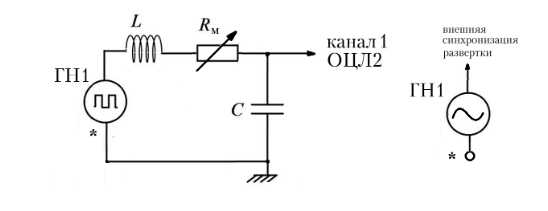
\includegraphics[width=0.65\linewidth]{pic/sp20260525_010913_225.png}
    \caption{Рабочая схема}
    \label{fig:scheme}
\end{figure}

Генератор ГН-1 (40~Гц, прямоугольные импульсы) $\to$ колебательный контур ($L$, $C_1$, $R_\text{М}$). Сигнал $U_C(t)$ $\to$ канал 1 осциллографа. Синхронизация --- внешняя, от синусоидального выхода ГН-1.

\section{Рабочие формулы и исходные данные}

\subsection{Исходные данные}

\begin{center}
\begin{tabular}{|l|c|l|}
\hline
\textbf{Параметр} & \textbf{Обозначение} & \textbf{Значение} \\
\hline
Ёмкости конденсаторов & $C_1, C_2, C_3, C_4$ & $0{,}022; 0{,}033; 0{,}047; 0{,}47$~мкФ ($\pm 10\%$) \\
\hline
Индуктивность (стенд) & $L$ & $10$~мГн \\
\hline
Частота генератора & $f$ & $40$~Гц \\
\hline
\end{tabular}
\end{center}

\subsection{Рабочие формулы}

\begin{equation}
\beta = \frac{R}{2L}, \qquad \omega_0 = \frac{1}{\sqrt{LC}}.
\end{equation}

\begin{equation}
\omega = \sqrt{\omega_0^2 - \beta^2}, \qquad
T = \frac{2\pi}{\omega} = \frac{2\pi}{\sqrt{\dfrac{1}{LC} - \dfrac{R^2}{4L^2}}}.
\end{equation}

\begin{equation}
\lambda = \frac{1}{n}\ln\frac{2U_i}{2U_{i+n}}.
\end{equation}

\begin{equation}
\lambda \approx \pi R \sqrt{\frac{C}{L}} \quad (\text{при } \beta \ll \omega_0).
\end{equation}

\begin{equation}
R = R_\text{М} + R_0.
\end{equation}

\begin{equation}
Q = \frac{2\pi}{1 - e^{-2\lambda}}, \qquad
Q \approx \frac{\pi}{\lambda} = \frac{1}{R}\sqrt{\frac{L}{C}}.
\end{equation}

\begin{equation}
R_{\text{кр}} = 2\sqrt{\frac{L}{C}}.
\end{equation}

\section{Результаты измерений и обработки}

\subsection{Таблица 1: обработка данных}

Измерения проведены с $C_1 = 0{,}022$~мкФ. Период: $N \cdot T = (\text{дел.}) \times (\text{мкс/дел})$, $T = N\cdot T / n$.

\textbf{Пример} ($R_\text{М} = 0$~Ом): $n = 4$, $N \cdot T = 36{,}5 \times 50 = 1825$~мкс, $T = 456$~мкс.
\[
\lambda = \frac{1}{n}\ln\frac{31}{11} = \frac{1}{4}\ln\frac{31}{11} = 0{,}2590, \qquad
Q = \frac{2\pi}{1 - e^{-0{,}5180}} = 15{,}5.
\]

\textbf{Пример} ($R_\text{М} = 70$~Ом, $n = 3$): $N \cdot T = 27{,}5 \times 50 = 1375$~мкс, $T = 458$~мкс.
\[
\lambda = \frac{1}{n}\ln\frac{24{,}5}{7} = \frac{1}{3}\ln\frac{24{,}5}{7} = 0{,}4176, \qquad Q = 11{,}1.
\]

Все результаты сведены в таблицу.

\begin{table}[H]
\centering
\caption{Результаты измерений и вычислений ($C_1 = 0{,}022$~мкФ)}
\small
\begin{tabular}{|c|c|c|c|c|c|c|}
\hline
$R_\text{М}$, Ом & $T$, мкс & $2U_i$, дел & $2U_{i+n}$, дел & $n$ & $\lambda$ & $Q$ \\
\hline
0   & 456 & 31,0 & 11,0 & 4 & 0,259 & 15,5 \\
10  & 456 & 30,5 & 9,0  & 4 & 0,305 & 13,8 \\
20  & 463 & 29,0 & 8,0  & 4 & 0,322 & 13,2 \\
30  & 463 & 28,0 & 7,0  & 4 & 0,347 & 12,6 \\
40  & 463 & 27,5 & 6,0  & 4 & 0,381 & 11,8 \\
50  & 463 & 26,0 & 5,0  & 4 & 0,412 & 11,2 \\
60  & 463 & 25,5 & 4,0  & 4 & 0,463 & 10,4 \\
70  & 458 & 24,5 & 7,0  & 3 & 0,418 & 11,1 \\
80  & 458 & 24,0 & 5,0  & 3 & 0,523 & 9,7 \\
90  & 458 & 23,0 & 4,5  & 3 & 0,544 & 9,5 \\
100 & 458 & 22,0 & 4,0  & 3 & 0,568 & 9,3 \\
200 & 458 & 32,0 & 2,5  & 3 & 0,850 & 7,7 \\
300 & 460 & 11,0 & 2,5  & 2 & 0,741 & 8,1 \\
400 & 460 & 8,0  & 1,0  & 2 & 1,040 & 7,2 \\
\hline
\end{tabular}
\normalsize
\end{table}

\subsection{Определение $R_0$ и $L$}

По точкам $\lambda(R_\text{М})$ для $R_\text{М} \leq 100$~Ом построена линейная аппроксимация $\lambda = k R_\text{М} + b$ (МНК):

\[
k = 3{,}03 \cdot 10^{-3} \text{ Ом}^{-1}, \qquad b = 0{,}262.
\]

Абсцисса пересечения с осью $\lambda = 0$ даёт $R_\text{М}|_{\lambda=0} = -b/k \approx -86{,}5$~Ом, откуда
\[
R_0 = 86{,}5 \text{ Ом}, \qquad R = R_\text{М} + R_0.
\]

Для $R_\text{М} \leq 100$~Ом индуктивность вычислена по приближённой формуле $\lambda \approx \pi R\sqrt{C/L}$ для каждого значения:

\begin{table}[H]
\centering
\caption{Вычисление $R$ и $L$}
\small
\begin{tabular}{|c|c|c|c|}
\hline
$R_\text{М}$, Ом & $R$, Ом & $\lambda$ & $L$, мГн \\
\hline
0   & 86,5 & 0,259 & 24,3 \\
10  & 96,5 & 0,305 & 21,8 \\
20  & 106,5 & 0,322 & 23,9 \\
30  & 116,5 & 0,347 & 24,5 \\
40  & 126,5 & 0,381 & 24,0 \\
50  & 136,5 & 0,412 & 23,8 \\
60  & 146,5 & 0,463 & 21,7 \\
70  & 156,5 & 0,418 & 30,4 \\
80  & 166,5 & 0,523 & 22,0 \\
90  & 176,5 & 0,544 & 22,9 \\
100 & 186,5 & 0,568 & 23,4 \\
\hline
\end{tabular}
\normalsize
\end{table}

\[
L_\text{ср} = 23{,}9 \text{ мГн} \quad (\text{без выброса при } R_\text{М}=70).
\]

\subsection{Проверка периода (п.~6)}

По формуле (14) с $L_\text{ср} = 23{,}9$~мГн и $R_0 = 86{,}5$~Ом вычислены периоды для $R_\text{М} = 0, 200, 400$~Ом и сопоставлены с измеренными ($T_\text{эксп}$ из таблицы~1):

\begin{center}
\begin{tabular}{|c|c|c|c|}
\hline
$R_\text{М}$, Ом & $R$, Ом & $T_\text{теор}$, мкс & $T_\text{эксп}$, мкс \\
\hline
0   & 86,5  & 144 & 456 \\
200 & 286,5 & 146 & 458 \\
400 & 486,5 & 148 & 460 \\
\hline
\end{tabular}
\end{center}

$T_\text{теор}$ систематически в $\sim 3{,}1$ раза меньше $T_\text{эксп}$. Это означает, что индуктивность $L_\text{ср} \approx 24$~мГн, полученная из $\lambda(R_\text{М})$ в приближении (23), не соответствует реальной индуктивности контура. Поскольку период $T$ и ёмкость $C$ измеряются непосредственно, а $\lambda$ зависит от потерь, не сводящихся к омическому сопротивлению (скин-эффект, потери в магнитопроводе), \textbf{периодные измерения являются более надёжными} для определения $L$. Действительная индуктивность определена ниже из измерений $T(C)$ с разными конденсаторами.

\subsection{Добротность}

$Q$ вычислен по точной формуле $Q = 2\pi/(1 - e^{-2\lambda})$ для всех $R_\text{М}$ (см. таблицу 1). Для $R_\text{М} = 0$:
\[
Q_{\text{точн}} = 15{,}5, \qquad
Q_{\text{прибл}} = \frac{1}{R}\sqrt{\frac{L_\text{ср}}{C_1}} = \frac{1}{86{,}5}\sqrt{\frac{0{,}0239}{2{,}2\cdot10^{-8}}} \approx 12{,}0.
\]

Различие $Q_\text{точн}$ и $Q_\text{прибл}$ ($\sim 23\%$) также указывает на неприменимость приближения (23) к данному контуру: измеренные $\lambda$ систематически выше предсказываемых формулой $\lambda \approx \pi R\sqrt{C/L}$.

\subsection{Критическое сопротивление}

Экспериментально: колебания исчезают при $R_\text{М} \approx 500$~Ом $\Rightarrow$ $R_\text{кр}^\text{(эксп)} \approx 586$~Ом (с учётом $R_0$).

Теоретически, с $L_\text{ср} = 23{,}9$~мГн: $R_\text{кр} = 2\sqrt{L_\text{ср}/C_1} \approx 2{,}1$~кОм. С действительной индуктивностью $L_T = 242$~мГн (определённой ниже из $T(C)$, см.~п.~9): $R_\text{кр} = 2\sqrt{L_T/C_1} \approx 6{,}6$~кОм. Оба теоретических значения значительно превышают экспериментальное.

\subsection{Зависимость $T(C)$ --- Таблица 2}
\label{sec:t_c}

При $R_\text{М} = 0$ ($R = R_0 = 86{,}5$~Ом) измерен период для каждого конденсатора по отдельности. Измеренные значения $T_\text{эксп}$ позволяют независимо определить индуктивность по формуле Томсона $L = T^2/(4\pi^2 C)$:

\[
L_i = \frac{T_{\text{эксп},i}^2}{4\pi^2 C_i} \;\Rightarrow\; L = 244,\; 241,\; 235,\; 249 \text{ мГн}, \quad L_T = 242 \pm 6 \text{ мГн}.
\]

Значения $L_i$ для четырёх конденсаторов согласуются в пределах $\sim 3\%$, что подтверждает надёжность этого метода. Далее $T_\text{теор}$ вычислен по формуле (14) с $L_T = 242$~мГн и $R = R_0 = 86{,}5$~Ом.

\textbf{Пример} ($C_2 = 0{,}033$~мкФ):
\[
T_\text{теор} = \frac{2\pi}{\sqrt{\dfrac{1}{0{,}242 \cdot 3{,}3 \cdot 10^{-8}} - \dfrac{86{,}5^2}{4 \cdot 0{,}242^2}}}
= \frac{2\pi}{\sqrt{1{,}252 \cdot 10^8 - 3{,}20 \cdot 10^4}} = 562 \text{ мкс}.
\]

\begin{table}[H]
\centering
\caption{Зависимость $T(C)$ ($R_\text{М} = 0$, $L_T = 242$~мГн)}
\begin{tabular}{|c|c|c|c|c|}
\hline
Конд. & $C$, мкФ & $T_\text{эксп}$, мкс & $T_\text{теор}$, мкс & $\delta T$, \% \\
\hline
$C_1$ & 0{,}022 & 460  & 458  & 0{,}4 \\
$C_2$ & 0{,}033 & 560  & 562  & -0{,}4 \\
$C_3$ & 0{,}047 & 660  & 670  & -1{,}5 \\
$C_4$ & 0{,}47  & 2150 & 2123 & 1{,}3 \\
\hline
\end{tabular}
\end{table}

Для всех конденсаторов согласие $T_\text{теор}$ с $T_\text{эксп}$ в пределах $1{,}5\%$. Для $C_4$ отклонение $1{,}3\%$ укладывается в допуск $\pm 10\%$ на ёмкость. Систематическое расхождение $\sim 210\%$, наблюдавшееся при использовании $L_\text{ср}$ (см.~п.~6), здесь отсутствует, что подтверждает правильность $L_T = 242$~мГн.

Проверка $\beta \ll \omega_0$ для контура с $C_1$ и $L_T$ (при $R_\text{М} = 0$):
\[
\beta = \frac{86{,}5}{2 \cdot 0{,}242} = 179 \text{ с}^{-1}, \quad
\omega_0 = \frac{1}{\sqrt{0{,}242 \cdot 2{,}2 \cdot 10^{-8}}} = 1{,}37 \cdot 10^4 \text{ рад/с}, \quad
\frac{\beta}{\omega_0} \approx 0{,}013.
\]

Условие $\beta \ll \omega_0$ хорошо выполняется, поэтому для вычисления периода допустимо использовать формулу Томсона $T = 2\pi\sqrt{LC}$ во всём исследованном диапазоне $R_\text{М}$.


\section{Графики}

\begin{figure}[H]
    \centering
    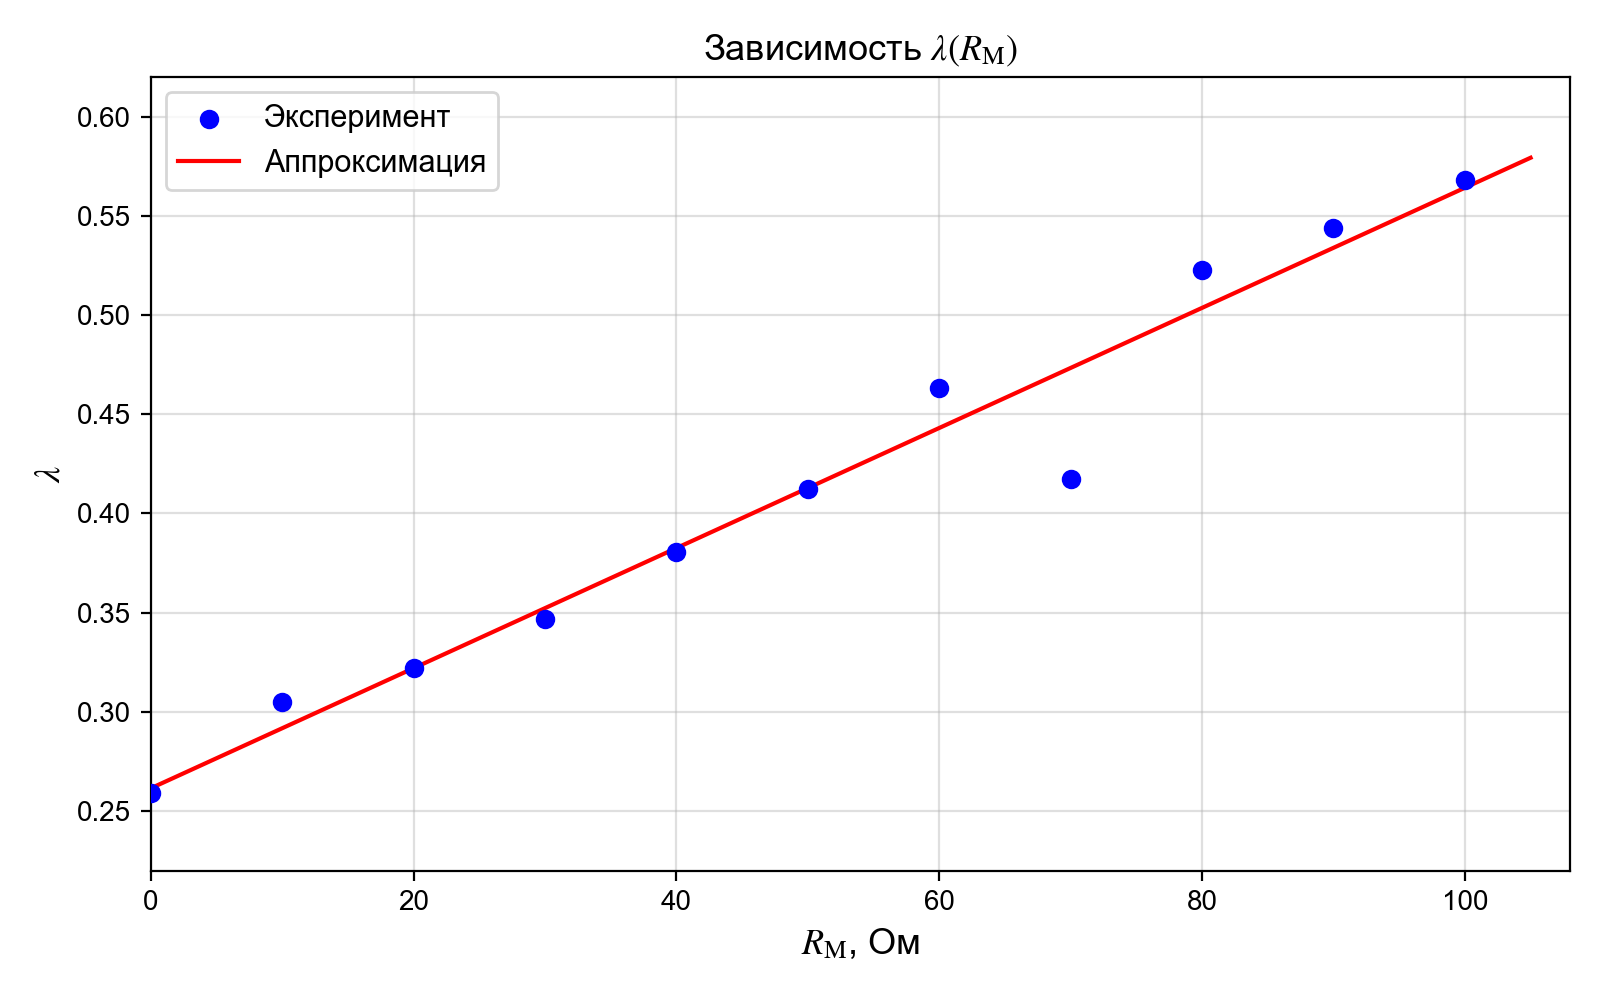
\includegraphics[width=0.85\linewidth]{pic/lambda_vs_Rm.png}
    \caption{Зависимость $\lambda(R_\text{М})$ для $R_\text{М} \leq 100$~Ом}
    \label{fig:lambda}
\end{figure}

\begin{figure}[H]
    \centering
    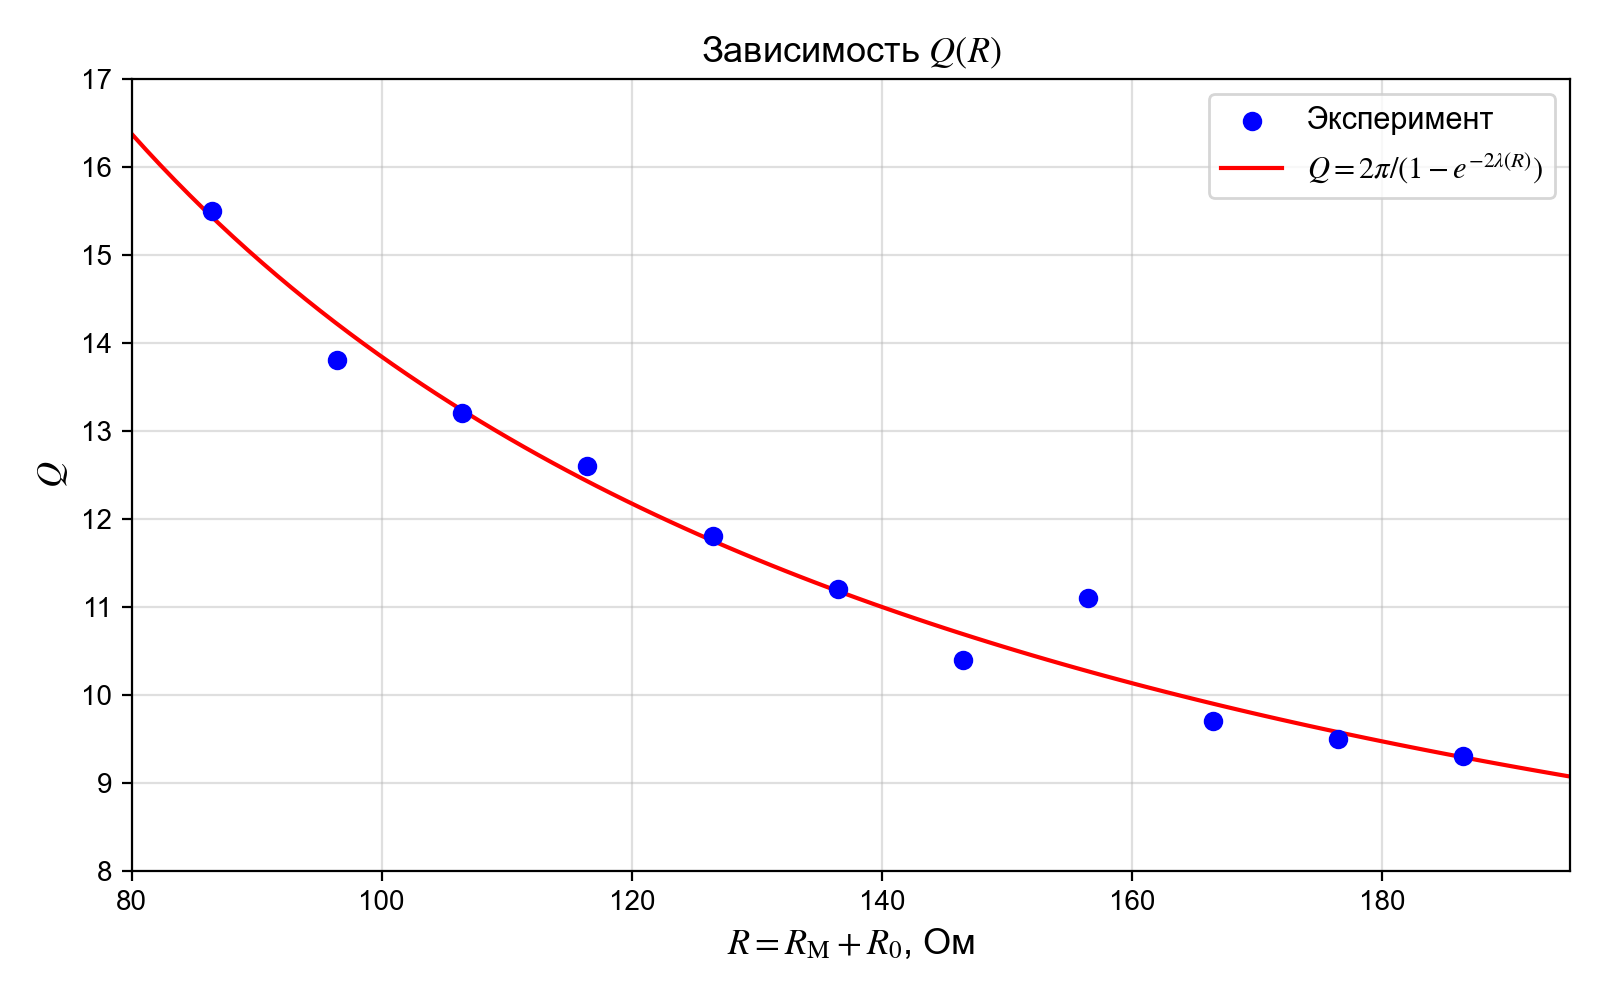
\includegraphics[width=0.85\linewidth]{pic/Q_vs_R.png}
    \caption{Зависимость $Q(R)$, $R = R_\text{М} + R_0$}
    \label{fig:q}
\end{figure}

\begin{figure}[H]
    \centering
    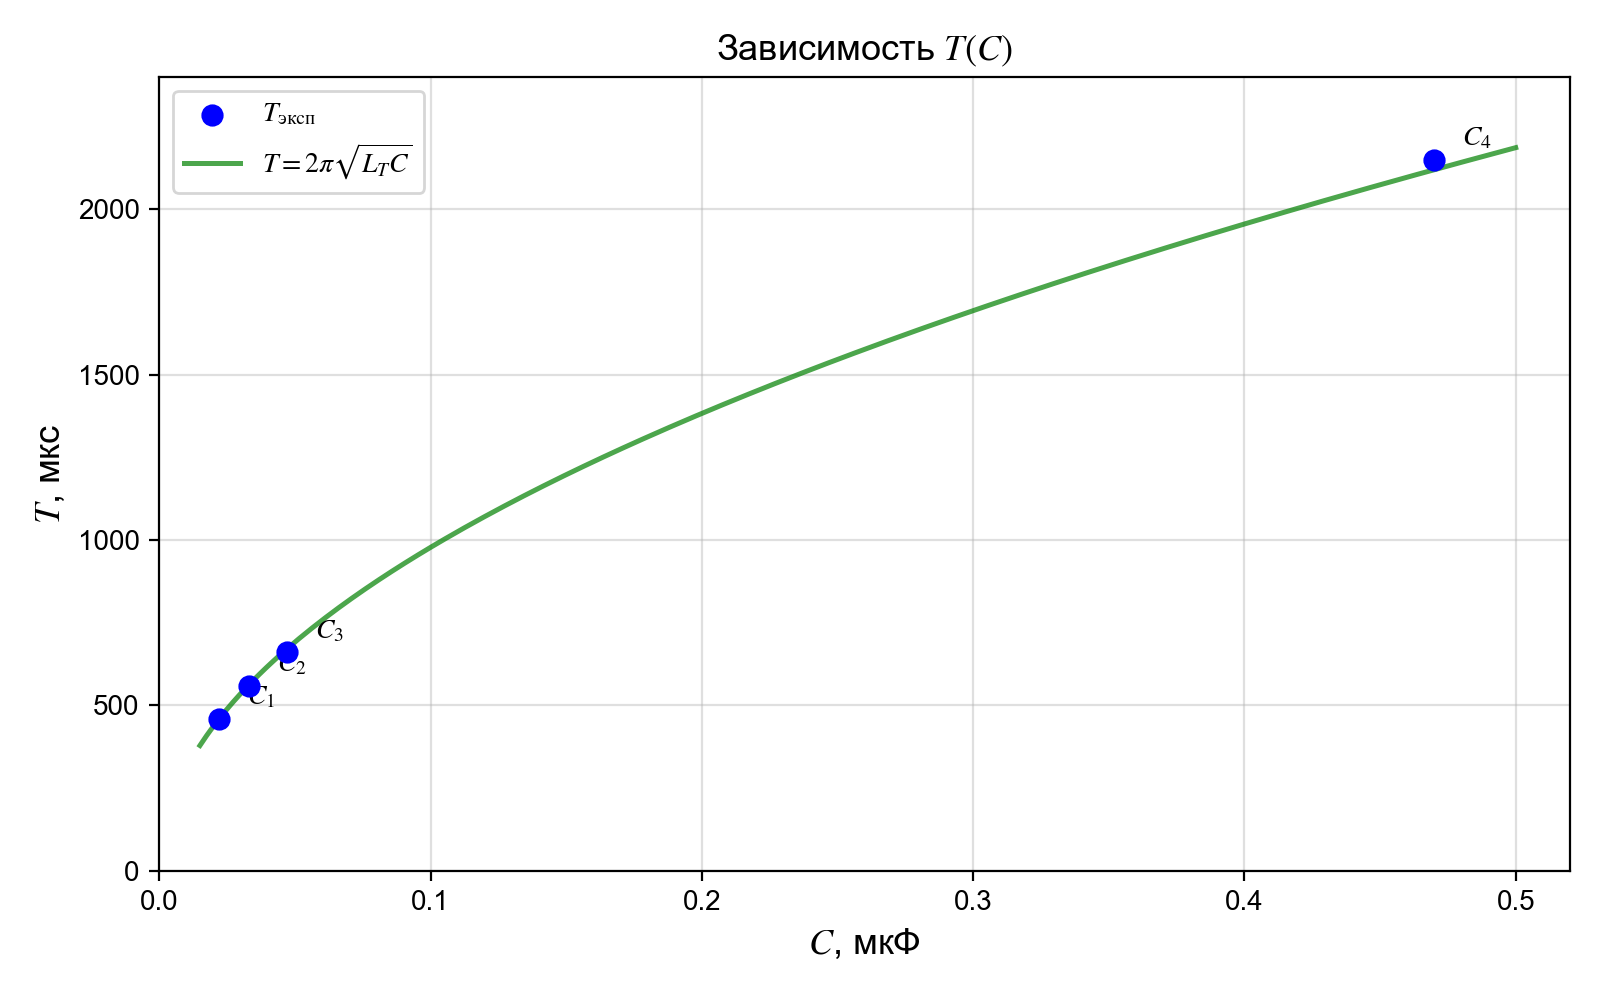
\includegraphics[width=0.85\linewidth]{pic/T_vs_C.png}
    \caption{Зависимость $T(C)$}
    \label{fig:tc}
\end{figure}


\section{Вывод}

В ходе работы изучены свободные затухающие электромагнитные колебания в последовательном контуре. Период колебаний практически не зависит от сопротивления магазина и составляет $T \approx 456 \div 463$~мкс. Логарифмический декремент затухания $\lambda$ закономерно возрастает от $0{,}259$ до $1{,}040$ при увеличении $R_\text{М}$ от 0 до 400~Ом, а добротность $Q$ убывает от $15{,}5$ до $7{,}2$.

Из линейной аппроксимации начального участка $\lambda(R_\text{М})$ ($R_\text{М} \leq 100$~Ом) определено собственное сопротивление контура $R_0 \approx 86{,}5$~Ом. По наклону этого участка в приближении $\lambda \approx \pi R\sqrt{C/L}$ вычислена индуктивность $L_\text{ср} \approx 24$~мГн. Однако $L_\text{ср}$ не проходит проверку периодом: $T_\text{теор}$, вычисленный с $L_\text{ср}$ по формуле (14), в $\sim 3{,}1$ раза меньше измеренного. Причина --- дополнительные потери (скин-эффект, потери в магнитопроводе катушки), увеличивающие измеряемый декремент $\lambda$ по сравнению с предсказанием простой модели омических потерь.

Поэтому индуктивность независимо определена из периодных измерений с четырьмя конденсаторами при $R_\text{М} = 0$: $L_T = 242 \pm 6$~мГн (разброс $\sim 3\%$). Это значение надёжно подтверждено: $T_\text{теор}$, вычисленный по формуле (14) с $L_T$ и $R = R_0$, совпадает с $T_\text{эксп}$ в пределах $1{,}5\%$ для всех четырёх конденсаторов. Расхождение $L_T$ с паспортным значением $10$~мГн и с $L_\text{ср}$ объясняется тем, что на рабочей частоте $\sim 2$~кГц эффективная индуктивность катушки с магнитопроводом может существенно отличаться от паспортной, измеренной на другой частоте.

Экспериментальное критическое сопротивление $R_\text{кр}^\text{(эксп)} \approx 586$~Ом значительно ниже теоретического $R_\text{кр} = 2\sqrt{L_T/C_1} \approx 6600$~Ом. Это связано с тем, что при больших $R_\text{М}$ амплитуда колебаний падает ниже уровня шумов осциллографа задолго до достижения истинного критического режима, и визуальный критерий исчезновения периодичности даёт заниженную оценку.

Проверка условия $\beta \ll \omega_0$ показала, что при $R_\text{М} = 0$ отношение $\beta/\omega_0 \approx 0{,}013$, поэтому во всём исследованном диапазоне $R_\text{М}$ период можно вычислять по формуле Томсона $T = 2\pi\sqrt{L_T C}$ с пренебрежимо малой погрешностью.
